\chapter{tikz/pgf作图}
\definecolor{spec}{rgb}{.121,.562,.996}


\section{基本图元}

\begin{tkzexample}[code only,small,num]
\begin{tikzpicture}[scale=4]

\coordinate (O) at (0,0,0);
\coordinate (X) at (1,0,0);
\coordinate (P) at (0.7071,0.7071,0);
 \draw[domain=-2:2,samples=100,smooth];
 {\draw[color=black,thick,->] (0,0,0) -- (2,0,0) node[anchor=north east]{$x$};}%  
    {\draw[color=black,thick,->] (0,0,0) -- (0,2,0) node[anchor=north west]{$y$};}%  
    {\draw[color=black,thick,->] (0,0,0) -- (0,0,2) node[anchor=south]{$z$};}%  
    \draw[color=blue,thick,->] (0,0,0) -- (1,0,0) node[anchor = north west]{$P(1,0,0)$};
     \draw[color=red,thick,->] (0,0,0) -- (0.7071,0.7071,0) node[anchor = south west]{$P'$};
\draw [thick, dashed] (0,0.7071,0) node[left] {$(0,1/\sqrt{2},0)$} -- (0.7071,0.7071,0)
   -- (0.7071,0,0) node[anchor=north]{$(1/\sqrt{2},0,0)$};
 pic ["$\theta$",draw,->] {angle = X--O--P};
\end{tikzpicture}
\end{tkzexample}



arc三元组定义(0:45:3mm)
表示从0度到45度,半径为3mm的圆弧
\begin{tikzpicture}[scale=4]

\coordinate (O) at (0,0,0);
\coordinate (X) at (1,0,0);
\coordinate (P) at (0.7071,0.7071,0);
 \draw[domain=-2:2,samples=100,smooth];
 {\draw[color=black,thick,->] (0,0,0) -- (2,0,0) node[anchor=north east]{$x$};}%  
    {\draw[color=black,thick,->] (0,0,0) -- (0,2,0) node[anchor=north west]{$y$};}%  
    {\draw[color=black,thick,->] (0,0,0) -- (0,0,2) node[anchor=south]{$z$};}%  
    \draw[color=blue,thick,->] (0,0,0) -- (1,0,0) node[anchor = north west]{$P(1,0,0)$};
     \draw[color=red,thick,->] (0,0,0) -- (0.7071,0.7071,0) node[anchor = south west]{$P'$};
\draw [thick, dashed] (0,0.7071,0) node[left] {$(0,1/\sqrt{2},0)$} -- (0.7071,0.7071,0)
   -- (0.7071,0,0) node[anchor=north]{$(1/\sqrt{2},0,0)$};

\shadedraw[left color=gray,right color=green, draw=green!50!black] (0,0) -- (3mm,0mm) arc (0:45:3mm) node[anchor = north west]{$45^{\circ}$} -- cycle; 
   
\end{tikzpicture}

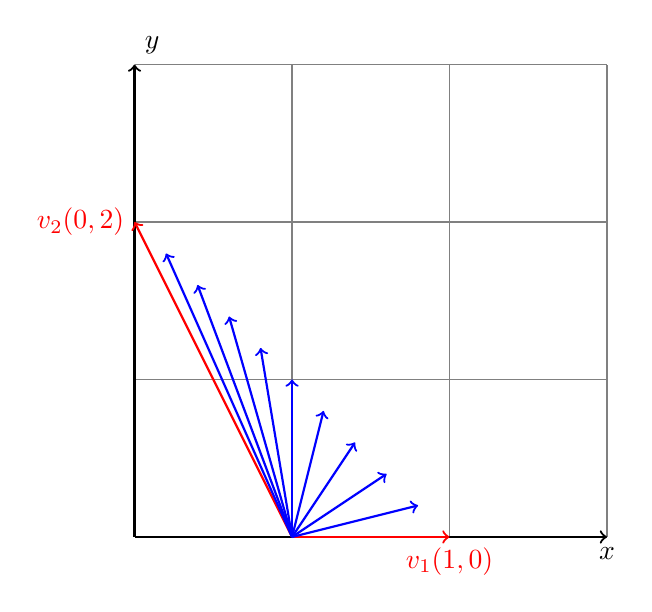
\begin{tikzpicture}[scale=2]
\draw[thin, color = gray] (0,0) grid (3,3);
\draw[thick,->] (0,0) -- (0,3) node [anchor = south west]{$y$};
\draw[thick,->]  (0,0) -- (3,0) node [anchor = north] {$x$};
\draw[thick,color = red, ->] (1,0) -- (2,0) node [anchor = north] {$v_1(1,0)$};
\draw[thick,color =red ,->]  (1,0) -- (0,2) node[anchor = east] {$v_2(0,2)$};
\foreach \t in {0.1,0.2, 0.3,0.4,0.5,0.6,0.7,0.8,0.9}
	\draw[thick,color = blue, ->] (1,0) -- (2-2*\t,2*\t);
\end{tikzpicture}

填充用法:
\begin{tkzexample}[code only,small,num]
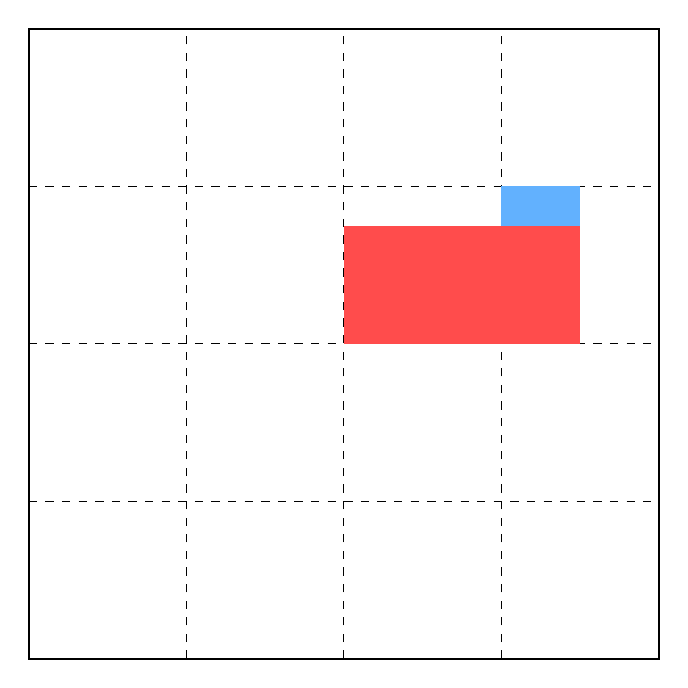
\begin{tikzpicture}[scale=0.5]
\draw [thick] (0,0)--(16,0);
\draw[step=4,dashed] (0,0) grid (16,16);
\draw[thick] (0,0) rectangle (16,16);

\fill[spec!70] (12, 8) rectangle +(2,4);
\fill[red!70] (8,8) rectangle +(6,3);
\end{tikzpicture}
\end{tkzexample}
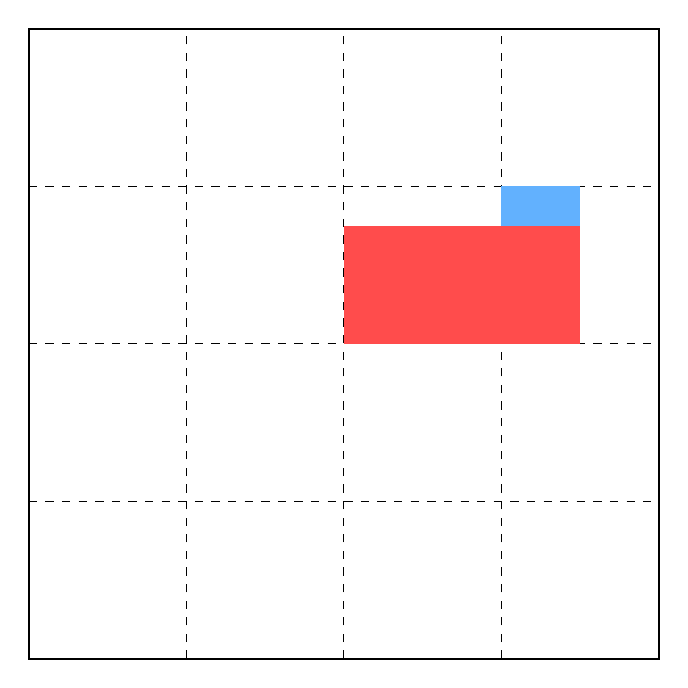
\begin{tikzpicture}[scale=0.5]
\draw [thick] (0,0)--(16,0);
\draw[step=4,dashed] (0,0) grid (16,16);
\draw[thick] (0,0) rectangle (16,16);

\fill[spec!70] (12, 8) rectangle +(2,4);
\fill[red!70] (8,8) rectangle +(6,3);
\end{tikzpicture}


 
\begin{tikzpicture}  
    %\draw [thin,red,smooth,domain=0:6.5] plot[id=x] function{sin(2*x)*exp(-x/4)};  
    %\draw[ycomb,gray,line width=0.3cm] plot coordinates {(1,1) (2,2) (3,3)};  
  
    \filldraw[black,thick] (5,1) circle (3);  
    \filldraw[white] (5,-0.5) circle(1.5);  
    \begin{scope}  
      \clip (5,1) circle (3);  
      \filldraw[white] (5,-2) rectangle (8,4);  
      \filldraw[black] (5,2.5) circle (1.5);  
    \end{scope}  
    \filldraw[white] (5,2.5) circle (0.2cm);  
    \filldraw[black] (5,-0.5) circle (0.2cm);  
  \end{tikzpicture}  


\section{数学计算}
 because TikZ only accepts fully expandable input\\
 The $\backslash $pgfmathparse macro is not expandable and can't be used inside coordinates. Placing $\backslash$ pgfmathresult 
 behind it, like $\backslash$ pgfmathresult, which is expandable in the coordinates\\
 然后,就是sin,cos函数默认是以角度为参数的,想要弧度为参数的话使用sin(x r),r代表使用弧度\\
 对foreach循环中的变量进行计算,可以参考如下链接提供的方法:
 \href{stackexchange}{http://tex.stackexchange.com/questions/132982/numbering-nodes-in-a-for-loop}
 或者参考我的代码:
 getx与setx的方法都是定义宏,但是getx把返回值也作为一个参数传进去了
 %\begin{tkzexample}[code only,small,num]
 \begin{tikzpicture}[scale=1]

\pgfmathparse{0.5*sin(4.5/180*pi)}\let\b=\pgfmathresult
\newcommand{\getx}[2]{
 \pgfmathparse{cos(#2*4.5/180*pi)}\let#1\pgfmathresult
}
\newcommand{\setx}[1]{cos(#1*4.5/180*pi)}
%\getx[1]\let\a = \pgfmathresult
\draw[->,thick] (0,0) -- (4cm,0);
\draw[->,thick] (0,0) -- (0,4cm);
\draw (0,0) circle [radius = 4cm];
\foreach \x  [evaluate={\tmpx=4*cos(\x*4.5)},evaluate={\tmpy=2*sin(\x*4.5)}] in {0,2,...,40}
{
	 %\getx \tmpa{\x}
	 %\pgfmathparse{cos(\x* 4.5/180*pi)}
	% \draw (0,0) circle( \tmpx );
	 \fill[color=red] ( {\tmpx}, \tmpy) circle(1pt);
	 \draw[->,thick,color =blue] (\tmpx, \tmpy) -- ( 1.5*\tmpx,1.5*\tmpy) ;
	 %\draw[->,thick,color =red] (\tmpx, \tmpy) -- ( 1.5*\tmpx, 6*\tmpy) ;
}
\foreach \y in {1cm,2cm,3cm,4cm}
	\draw (-1pt, \y) -- (1pt,\y);
\end{tikzpicture}
 %\end{tkzexample}
